\part{Variables in GLSL}
\frame{\partpage}

\begin{frame}{Passing values from the application to the shader}
	There are two ways:
	\begin{itemize}
		\pause\item \textbf{Vertex attributes}
			\begin{itemize}
				\pause\item Different values for each vertex
				\pause\item More on this later in the module
			\end{itemize}
		\pause\item \textbf{Uniform variables}
			\begin{itemize}
				\pause\item Constant across one \lstinline{glDraw...} call
			\end{itemize}
	\end{itemize}
\end{frame}

\begin{frame}[fragile]{Uniform variables}
	\pause In GLSL (outside \lstinline{main()}):
	\begin{lstlisting}
uniform vec3 myVariable;
	\end{lstlisting}
	\pause In C++:
	\begin{lstlisting}[language=C++]
GLuint location
  = glGetUniformLocation(programID, "myVariable");
	\end{lstlisting}
	\pause and then:
	\begin{lstlisting}[language=C++]
glUniform3f(location, 1, 2, 3);
	\end{lstlisting}
\end{frame}

\begin{frame}{Uniform variables}
	\begin{itemize}
		\pause\item \lstinline[language=C++]{glGetUniformLocation} is expensive --- do it on initialisation, not in the main loop
		\pause\item Uniforms can be any GLSL type...
		\pause\item ... but you must use the \lstinline[language=C++]{glUniform...} function that matches the type
	\end{itemize}
\end{frame}

\begin{frame}[fragile]{Passing values from the vertex shader to the fragment shader}
	\pause Define an \lstinline{out} variable in the vertex shader:
	\pause \begin{lstlisting}
out vec4 myVariable;
	\end{lstlisting}
	\pause Define an \lstinline{in} variable \textbf{of the same name} in the fragment shader:
	\pause \begin{lstlisting}
in vec4 myVariable;
	\end{lstlisting}
\end{frame}

\begin{frame}{Interpolation}
	\begin{columns}
		\begin{column}{0.5\textwidth}
			\begin{itemize}
				\pause\item The vertex shader sets a value for each vertex
				\pause\item So what is the value in the middle of the triangle?
				\pause\item The GPU \textbf{interpolates} the value across the triangle
			\end{itemize}
		\end{column}
		\begin{column}{0.45\textwidth}
			\pause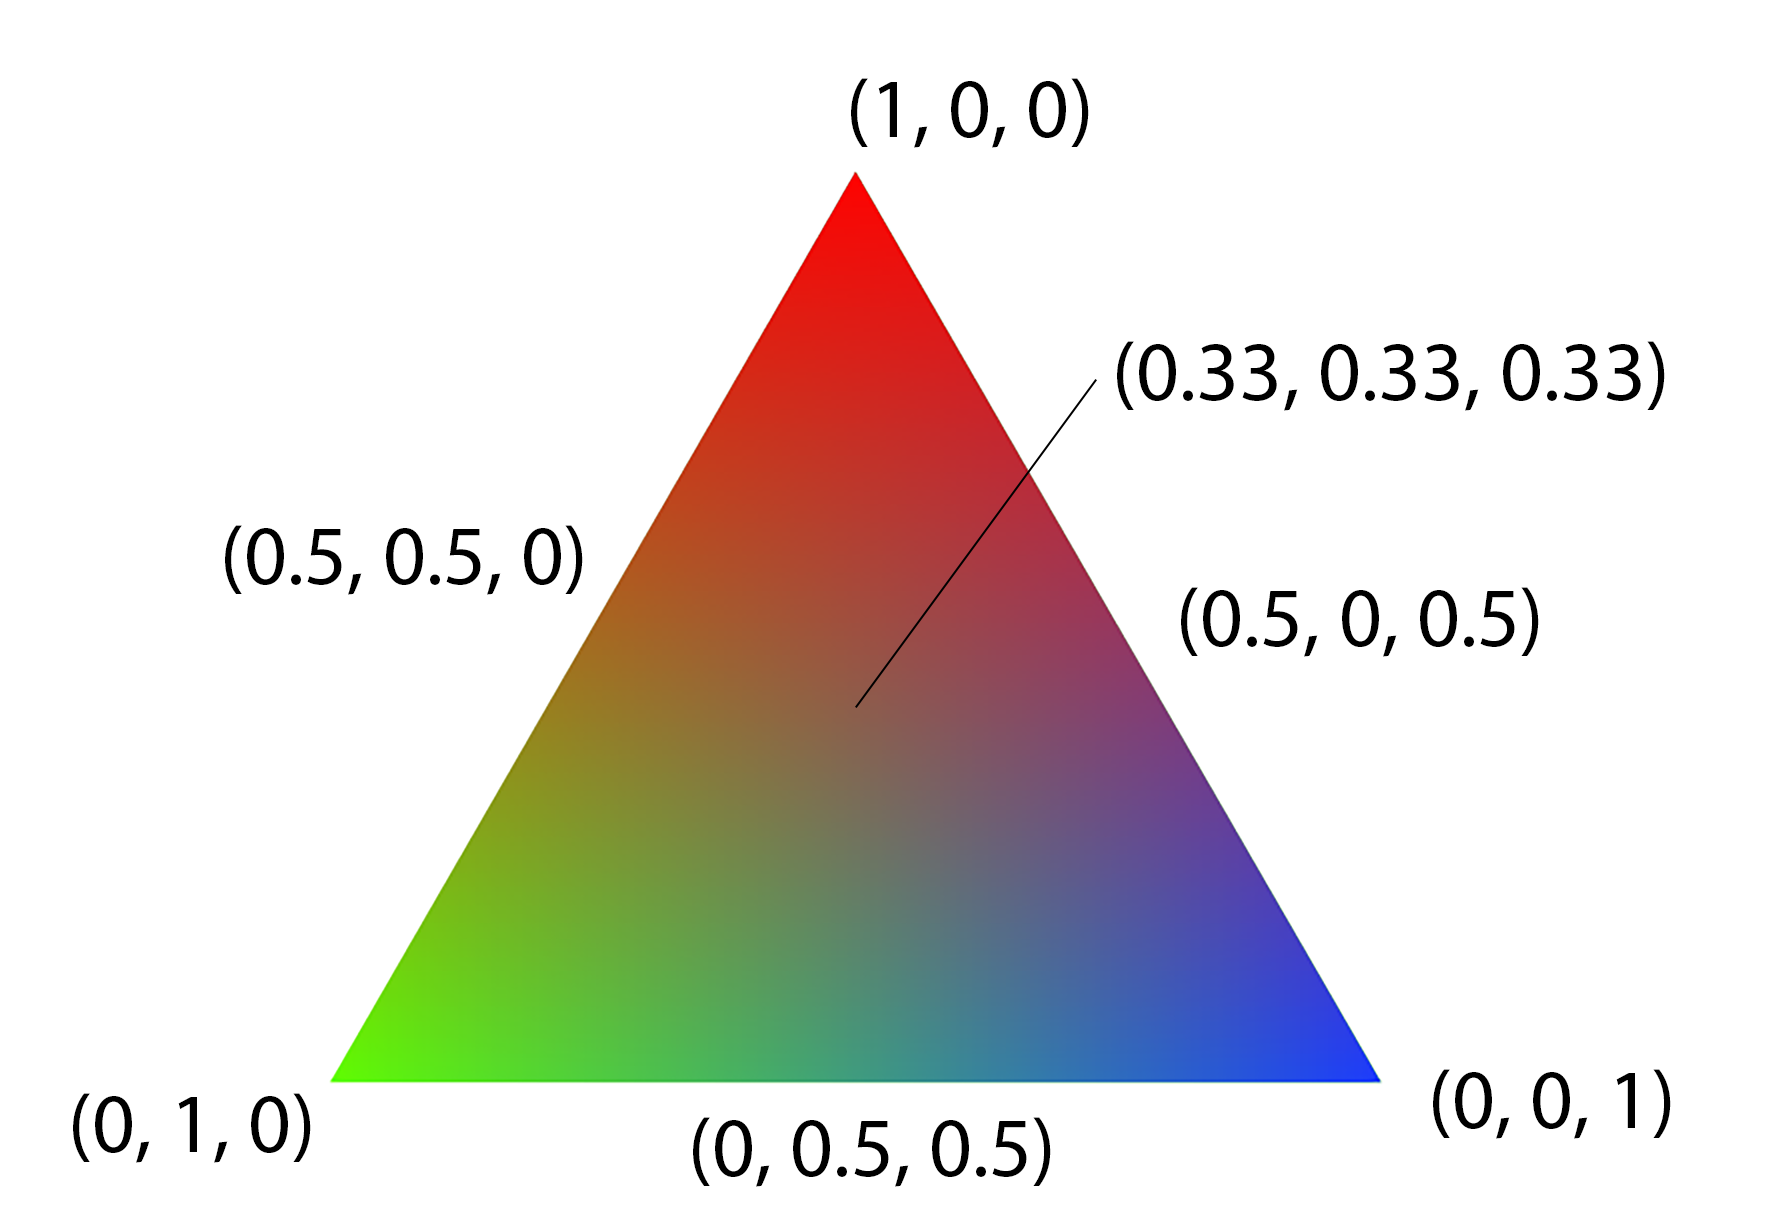
\includegraphics[width=\textwidth]{interpolation}
		\end{column}
	\end{columns}
\end{frame}
